% Provenance (never printed): old terminale S material on the Earth's internal
% heat (geothermal gradient and heat flow, radioactive heat production,
% conduction and convection, mantle convection, geothermal energy). Owner
% (Sync 0/1): heat flow, radiogenic heat production, secular cooling, thermal
% and mantle convection (recall the convection cell of Book 1 g8 first),
% geothermal energy. Geotherm and geothermal gradient are g11.03's; radioactivity,
% half-life, decay law and thermal conductivity are physics' (thermal
% conductivity used as "the rock's thermal conductivity k", never defined);
% hotspot track and plume g11.04's. Figures: figdata/grade-12/internal_heat.py.
\chapter{Panas Internal Bumi}\label{ch:g12:internal-heat}

Antara 1987 dan 1995, di dekat desa Windischeschenbach di Bavaria, para ahli
geologi mengebor sebuah lubang sedalam \qty{9101}{m} ke dalam \omterm{def:g12:continental-crust:continental-crust}{kerak benua}. Di
dasarnya batuan bersuhu sekitar \qty{265}{\celsius}, terlalu panas untuk dibor
lebih dalam lagi.
% ledger: gfz:ktb, gfz:ktb30

Dari sekitar \qty{10}{\celsius} di permukaan sampai \qty{265}{\celsius} pada
\qty{9.1}{km}, kenaikannya sekitar \qty{28}{\celsius} per kilometer, nilai yang
umum. Di mana pun di Bumi, suhu makin tinggi ke arah bawah, sehingga panas
terus-menerus mengalir keluar dari Bumi. Bab ini mengukur aliran itu,
menanyakan dari mana panas itu berasal, dan menunjukkan bagaimana panas itu
berpindah.
% values: ktb_gradient 28.0 (internal_heat.py, surface temperature taken as 10 degC); ledger: gfz:ktb (gradient about 28 K/km)

\begin{recall}
\omterm{def:g11:lithosphere-asthenosphere:geotherm}{Geoterm} adalah kurva suhu terhadap kedalaman di bawah suatu tempat, dan
\omterm{def:g11:lithosphere-asthenosphere:geotherm}{gradien geotermal} adalah kenaikan suhu per kilometer; lubang bor mengukur 25
sampai \qty{30}{\celsius} per kilometer di dekat permukaan
(\cref{ch:g11:lithosphere-asthenosphere}). Sebagian atom bersifat radioaktif:
atom-atom itu meluruh secara acak, jumlah yang tersisa berkurang separuhnya
setiap waktu paruh, dan setiap peluruhan melepaskan energi, yang akhirnya
menjadi panas (buku-buku fisika). Sel konveksi adalah lingkaran fluida yang
dipanaskan dari bawah, yang naik, menyebar, mendingin, dan tenggelam (Buku 1,
kelas 8). Di titik panas, sebuah lempeng bergerak di atas gumpalan mantel yang
panas (\cref{ch:g11:plate-motions}).
\end{recall}
% ledger: usgs:gradient-29 (Book 1 row)

\section{Gradien dan aliran panas}

\begin{definition}[Aliran panas]\label{def:g12:internal-heat:heat-flow}
Yang disebut \emph{aliran panas}\index{aliran panas} (atau fluks panas) di suatu
tempat adalah daya yang keluar dari bagian dalam Bumi melalui setiap meter
persegi permukaannya di tempat itu. Aliran panas diukur dalam miliwatt per
meter persegi (\unit{mW/m^2}).
\end{definition}
% ledger: b2dd10:continents

Panas mengalir dari yang panas ke yang dingin, dan makin curam gradien suhunya,
makin cepat panas itu mengalir. Seberapa banyak yang mengalir juga bergantung
pada batuannya: setiap batuan mempunyai konduktivitas termal $k$, dalam watt
per meter per kelvin, yang didefinisikan dalam buku-buku fisika.

\begin{proposition}[Aliran panas dan gradien]\label{prop:g12:internal-heat:fourier}
Melalui batuan berkonduktivitas termal $k$ yang suhunya naik terhadap
kedalaman dengan gradien $G$ (dalam kelvin per meter), \omterm{def:g12:internal-heat:heat-flow}{aliran panas} ke atas
menuju permukaan adalah
\[
  q = k\,G .
\]
\end{proposition}

Hukum konduksi ini, yang dikemukakan Fourier, di sini diterima tanpa bukti;
buku-buku fisika membuktikannya dalam bentuk umum.

\begin{method}[Aliran panas dari sebuah lubang bor]\label{met:g12:internal-heat:borehole}
\begin{enumerate}
  \item Ukurlah suhu pada beberapa kedalaman sebuah lubang bor, setelah lubang
        itu sempat kembali ke suhu batuannya.
  \item Plotkan suhu terhadap kedalaman dan ambillah kemiringannya: gradien
        $G$, yang diubah ke kelvin per meter.
  \item Ukurlah konduktivitas $k$ batuan itu pada inti bor di laboratorium.
  \item Kalikan: $q = kG$, dalam \unit{W/m^2}, lalu ubah ke \unit{mW/m^2}.
\end{enumerate}
\end{method}

\begin{example}[Sebuah lubang bor di granit]\label{ex:g12:internal-heat:borehole}
Sebuah lubang bor di granit yang konduktivitasnya \qty{2.72}{W/(m.K)}
mengukur gradien \qty{29}{\celsius} per kilometer, yaitu \qty{0.029}{K/m}.
Maka $q = 2.72 \times 0.029 \approx \qty{0.079}{W/m^2}$, sekitar
\qty{79}{mW/m^2}.
\end{example}
% ledger: roy:conductivity (granitic layer 6.5 mcal/(cm s degC) = 2.72 W/m/K), usgs:gradient-29 (Book 1 row)
% values: borehole_q_mW 78.9 (internal_heat.py)

Lebih dari 38\,000 pengukuran seperti itu telah digabungkan menjadi peta seluruh
Bumi. Benua-benua rata-rata kehilangan \qty{70.9}{mW/m^2}, dasar samudra
\qty{105.4}{mW/m^2}; di atas seluruh permukaan, \qty{91.6}{mW/m^2}.
Dikalikan dengan luas Bumi, \qty{5.101e14}{m^2}, jumlahnya
\[
  0.0916 \times \num{5.101e14} \approx \qty{4.67e13}{W} = \qty{46.7}{TW},
\]
sekitar 47 terawatt, plus minus 2.
% ledger: b2dd10:continents, b2dd10:half-space (47 +- 2 TW, 38,347 measurements)

Dasar samudra paling banyak kehilangan panas di tempat yang paling muda.
\omterm{def:g11:lithosphere-asthenosphere:lithosphere}{Litosfer} baru meninggalkan punggungan dalam keadaan panas, dan mendingin ketika
bergerak menjauh; \omterm{def:g12:internal-heat:heat-flow}{aliran panasnya} turun sebanding dengan satu per akar kuadrat
umurnya.

\begin{omfigure}
\begin{tikzpicture}
\begin{axis}[omrecord, width=0.72\linewidth, height=5.6cm, xmin=0, xmax=180, ymin=0, ymax=400,
  xlabel={umur dasar samudra (juta tahun)}, ylabel={aliran panas (\unit{mW/m^2})},
  xtick={0,30,...,180}, ytick={0,100,...,400}]
% computed in figdata/grade-12/internal_heat.py; ledger: b2dd10:half-space, b2dd10:continents
\addplot[omDef, line width=1.1pt, restrict x to domain=0:66.5] table[x=t_Myr, y=q] {figdata/out/grade-12-internal_heat-halfspace.dat};
\addplot[omDef, line width=1.1pt, densely dotted, restrict x to domain=66.5:180] table[x=t_Myr, y=q] {figdata/out/grade-12-internal_heat-halfspace.dat};
\addplot[omProp, line width=0.9pt, dashed, domain=0:180] {70.9};
\coordinate (lawlab) at (axis cs:14,250);
\coordinate (contlab) at (axis cs:100,80);
\end{axis}
\node[font=\scriptsize, text=omDef, anchor=west] at (lawlab) {$q = 490/\sqrt{t}$};
\node[font=\scriptsize, text=omProp, anchor=south west] at (contlab) {rata-rata benua, \qty{70.9}{mW/m^2}};
\end{tikzpicture}

{\small \omterm{def:g12:internal-heat:heat-flow}{Aliran panas} melalui dasar samudra terhadap umurnya, seperti yang
dihitung untuk pendinginan \omterm{def:g11:lithosphere-asthenosphere:lithosphere}{litosfer} ($t$ dalam juta tahun); di luar 66.5 juta
tahun (bertitik-titik) hukum itu diketahui kurang cocok. Sumber: Davies dan
Davies (2010).}
\end{omfigure}
% values: q_1Myr 490, q_10Myr 155, q_66.5Myr 60.1, age_where_q_equals_cont_Myr 47.8 (internal_heat.py)

\section{Dari mana panas itu berasal}

Panas itu mempunyai dua sumber. Yang pertama adalah radioaktivitas.

\begin{definition}[Produksi panas radiogenik]\label{def:g12:internal-heat:heat-production}
Yang disebut \emph{produksi panas radiogenik}\index{produksi panas radiogenik}
sebuah batuan adalah panas yang dilepaskan di dalamnya oleh peluruhan
atom-atom radioaktifnya, per satuan volume dan waktu, dalam mikrowatt per meter
kubik (\unit{\micro W/m^3}). Hampir semuanya berasal dari empat isotop:
uranium-238, uranium-235, torium-232, dan kalium-40.
\end{definition}
% ledger: dye12:isotopes, earle:heat-sources, kamland11:geonu

Unsur-unsur ini terpusat di dalam batuan \omterm{def:g12:continental-crust:continental-crust}{kerak benua}. Dari 2188 analisis,
produksi panas median granit adalah \qty{2.43}{\micro W/m^3}, basalt
\qty{0.21}{\micro W/m^3}, dan batuan ultramafik mantel hanya
\qty{0.11}{\micro W/m^3}, sekitar dua puluh kali lebih kecil daripada granit.
Lapisan granit setebal \qty{10}{km} menghasilkan
$2.43 \times 10^{-6} \times \num{10000} \approx \qty{0.024}{W}$ di bawah setiap
meter persegi, \qty{24}{mW/m^2}: sepertiga \omterm{def:g12:internal-heat:heat-flow}{aliran panas} benua-benua.
% ledger: b2vila:heat-production, b2dd10:continents
% values: granite_10km_mW 24.3, granite_over_ultramafic 21.9 (internal_heat.py)

Berapa banyak panas yang dihasilkan radioaktivitas di seluruh Bumi? KamLAND,
sebuah detektor bawah tanah di Jepang yang berisi 1000 ton cairan, menangkap
geoneutrino, yaitu antineutrino yang dilepaskan oleh peluruhan uranium dan
torium di dalam Bumi: detektor itu melihat yang pertama pada tahun 2005, dan
dalam 2135 hari perekaman, sekitar 106 geoneutrino di antara 841 peristiwa
kandidat. Dari hitungan itu, bersama hitungan sebuah detektor di Italia,
uranium-238 dan torium-232 bersama-sama melepaskan sekitar 20 terawatt.
Kalium-40 luput dari detektor; diketahui bahwa kalium-40 menambahkan sekitar
\qty{4}{TW}, dan uranium-235, yang diskalakan dari uranium-238, sekitar
\qty{0.4}{TW}. Jadi radioaktivitas memasok sekitar \qty{24}{TW}, kira-kira
separuh dari \qty{47}{TW} yang hilang dari Bumi.
% ledger: kamland11:geonu, dye12:isotopes, b2dd10:continents
% values: now_K40_TW 4.0, now_U235_TW 0.42, radiogenic_TW 24.4, share_radiogenic 0.523 (internal_heat.py)

\begin{definition}[Pendinginan sekuler]\label{def:g12:internal-heat:secular-cooling}
Yang disebut \emph{pendinginan sekuler}\index{pendinginan sekuler} Bumi adalah
hilangnya secara perlahan panas yang tersimpan di dalamnya sejak Bumi
terbentuk, yaitu panas primordial: bagian \omterm{def:g12:internal-heat:heat-flow}{aliran panas} yang tidak digantikan
oleh radioaktivitas, yang membuat mantel dan inti makin dingin dari zaman ke
zaman.
\end{definition}
% ledger: kamland11:geonu, earle:heat-sources

\begin{omfigure}
\begin{tikzpicture}
\begin{axis}[omrecord, xbar stacked, bar width=14pt, width=0.66\linewidth, height=3.2cm, scale only axis,
  xmin=0, xmax=50, ymin=0.4, ymax=2.6, ytick={1,2}, yticklabels={{sumber}, {kehilangan}},
  xlabel={daya (\unit{TW})}, ymajorgrids=false, legend columns=2, legend cell align=left,
  legend style={font=\scriptsize, at={(0.5,-0.42)}, anchor=north, /tikz/every even column/.append style={column sep=6pt}}]
% computed in figdata/grade-12/internal_heat.py; ledger: kamland11:geonu, dye12:isotopes, b2dd10:continents
\addplot[fill=omThm!55, draw=omThm] table[x=uth, y=bar] {figdata/out/grade-12-internal_heat-budget.dat};
\addplot[fill=omThm!25, draw=omThm] table[x=kuf, y=bar] {figdata/out/grade-12-internal_heat-budget.dat};
\addplot[fill=omDef!35, draw=omDef] table[x=secular, y=bar] {figdata/out/grade-12-internal_heat-budget.dat};
\addplot[fill=black!25, draw=black!60] table[x=surface, y=bar] {figdata/out/grade-12-internal_heat-budget.dat};
\legend{{uranium-238 dan torium-232 (geoneutrino)}, {kalium-40 dan uranium-235}, {pendinginan sekuler (sisanya)}, {aliran panas di permukaan}}
\end{axis}
\end{tikzpicture}

{\small Neraca panas Bumi saat ini: apa yang keluar dari permukaan (batang
atas) dan apa yang memasoknya (batang bawah). Sumber: KamLAND (2011); Davies
dan Davies (2010); Dye (2012).}
\end{omfigure}
% values: radiogenic_TW 24.4, secular_TW 22.3 (internal_heat.py)

Radioaktivitas lebih kuat pada masa lalu. Setiap isotop meluruh, sehingga
dahulu jumlahnya lebih banyak: satu waktu paruh ke belakang, dua kali lebih
banyak, dan dua kali lebih banyak panas. Mundur $t$ tahun mengalikan panas
sebuah isotop yang waktu paruhnya $T$ dengan $2^{t/T}$.

\begin{proposition}[Panas radiogenik pada masa lalu]\label{prop:g12:internal-heat:past}
Bila sebuah isotop yang waktu paruhnya $T$ melepaskan daya $H_0$ saat ini, maka
isotop itu melepaskan
\[
  H(t) = H_0 \, 2^{t/T} = H_0\, e^{\lambda t}, \qquad \lambda = \frac{\ln 2}{T},
\]
pada waktu $t$ yang lalu.
\end{proposition}

\begin{proof}
Daya itu sebanding dengan jumlah $N$ atom yang tersisa, karena setiap atom
meluruh dengan peluang yang sama per detik. Menurut hukum peluruhan, $N$
terbagi 2 setiap waktu paruh: $N_{\text{kini}} = N(t)\,2^{-t/T}$, sehingga $N(t) =
N_{\text{kini}}\,2^{t/T}$, dan dayanya mengikuti. Akhirnya $2^{t/T} =
e^{(t/T)\ln 2} = e^{\lambda t}$.
\end{proof}

\begin{omfigure}
\begin{tikzpicture}
\begin{axis}[omrecord, width=0.72\linewidth, height=6cm, xmin=0, xmax=4.5, ymin=0, ymax=120,
  x dir=reverse, xlabel={waktu sebelum sekarang (miliar tahun)}, ylabel={panas radiogenik (\unit{TW})},
  xtick={0,0.5,...,4.5}, ytick={0,20,...,120}, x tick label style={/pgf/number format/.cd, fixed, precision=1},
  legend pos=north east, legend style={font=\scriptsize}, legend cell align=left]
% computed in figdata/grade-12/internal_heat.py; ledger: kamland11:geonu, dye12:isotopes, nndc:halflives
\addplot[black, line width=1.2pt] table[x=t_Ga, y=total] {figdata/out/grade-12-internal_heat-past.dat};
\addplot[omThm, line width=0.9pt] table[x=t_Ga, y=U235] {figdata/out/grade-12-internal_heat-past.dat};
\addplot[omProp, line width=0.9pt, densely dashed] table[x=t_Ga, y=K40] {figdata/out/grade-12-internal_heat-past.dat};
\addplot[omDef, line width=0.9pt] table[x=t_Ga, y=U238] {figdata/out/grade-12-internal_heat-past.dat};
\addplot[omMeth, line width=0.9pt, densely dotted] table[x=t_Ga, y=Th232] {figdata/out/grade-12-internal_heat-past.dat};
\legend{total, uranium-235, kalium-40, uranium-238, torium-232}
\end{axis}
\end{tikzpicture}

{\small Panas yang dilepaskan oleh keempat isotop radioaktif mundur sampai
terbentuknya Bumi, yang dihitung dari nilai-nilai saat ini dengan hukum
peluruhan. Waktu paruh: torium-232, 14.0 miliar tahun; uranium-238, 4.468;
kalium-40, 1.248; uranium-235, 0.704.}
\end{omfigure}
% values: total_4.5Ga_TW 115.9, ratio_total_4.5Ga 4.75, ratio_U235_4.5Ga 84.0, ratio_K40_4.5Ga 12.2, share_U235_K40_4.5Ga 0.72 (internal_heat.py)

Empat setengah miliar tahun yang lalu, radioaktivitas melepaskan sekitar
\qty{116}{TW}, hampir lima kali nilai saat ini, dan sebagian besar berasal dari
uranium-235 dan kalium-40, dua isotop yang berumur pendek, yang sejak itu
hampir habis. Bumi muda jauh lebih panas di bagian dalamnya daripada sekarang.
% ledger: earle:heat-sources (radiogenic heat now roughly 25 % of what it was)

\section{Konduksi dan konveksi}

Panas hanya dapat melintasi zat padat secara konduksi, dari atom ke atom, dan
di dalam batuan proses itu sangat lambat. Panas melintasi jarak $L$ secara
konduksi dalam waktu sekitar $L^2/\kappa$, dengan $\kappa$, difusivitas termal
batuan, sekitar \qty{1e-6}{m^2/s}. Untuk mantel yang tebalnya
\qty{2891}{km},
\[
  \frac{(\num{2.891e6})^2}{\num{1e-6}} \approx \qty{8.4e18}{s} \approx
  \num{2.6e11} \text{ tahun},
\]
sekitar 260 miliar tahun, hampir enam puluh kali umur Bumi. Bila mantel hanya
menghantarkan panas secara konduksi, panas di kedalamannya masih akan hampir
seluruhnya ada di sana.
% ledger: england:kelvin (Book 3 row: kappa 1e-6 m2/s), data:prem (CMB at 2891 km)
% values: conduction_time_Gyr 264.9 (internal_heat.py)

Mantel itu padat, tetapi selama jutaan tahun ia merayap, sangat lambat, seperti
fluida yang sangat kaku: \omterm{def:g11:lithosphere-asthenosphere:lithosphere}{astenosfer} mengalir (\cref{ch:g11:lithosphere-asthenosphere}).
Jadi mantel kehilangan panasnya seperti udara di atas radiator, dengan
mengangkutnya.

\begin{definition}[Konveksi termal; konveksi mantel]\label{def:g12:internal-heat:convection}
Yang disebut \emph{konveksi termal}\index{konveksi termal} adalah perpindahan
panas oleh gerak bahan itu sendiri: bahan yang lebih hangat dan lebih ringan
naik, bahan yang lebih dingin dan lebih rapat tenggelam, seperti dalam sel
konveksi. Yang disebut \emph{konveksi mantel}\index{konveksi mantel} adalah
konveksi termal mantel Bumi yang padat, yang merayap beberapa sentimeter
setahun dan mengangkut panas bagian dalam Bumi menuju permukaan.
\end{definition}
% ledger: earle:heat-sources (solid mantle flows at centimetres a year)

Lempeng-lempeng adalah bagian atas konveksi ini. Di punggungan, mantel panas
naik dan ditambahkan pada lempeng; \omterm{def:g11:lithosphere-asthenosphere:lithosphere}{litosfer} mendingin ketika bergerak menjauh,
menjadi rapat, dan tenggelam oleh beratnya sendiri di \omterm{def:g11:subduction-zones:subduction}{zona subduksi}:
\omterm{def:g11:subduction-zones:slab}{lempengan-lempengan} adalah bagian aliran yang dingin dan tenggelam, dan citra
seismik menunjukkan \omterm{def:g11:subduction-zones:slab}{lempengan-lempengan} itu tenggelam jauh ke dalam mantel.
Gumpalan batuan panas diduga naik di bawah titik panas dari bagian dalam
mantel, mungkin dari tepat di atas inti.
% ledger: dye12:bse, earle:plume

\begin{omfigure}
\begin{tikzpicture}[x=1cm, y=1cm, font=\scriptsize]
  % mantle annulus sector
  \fill[omLithPeridotite!40] (0,0) ++(20:6.4) arc (20:160:6.4) -- ++(160:-3.2) arc (160:20:3.2) -- cycle;
  \fill[black!45] (0,0) ++(20:3.2) arc (20:160:3.2) -- (0,0) -- cycle;
  \node[white] at (0,1.6) {inti};
  % lithosphere
  \fill[black!15, draw=black!50] (0,0) ++(20:6.4) arc (20:160:6.4) -- ++(160:-0.3) arc (160:20:6.1) -- cycle;
  % ridge (top) and two trenches
  \draw[omThm, line width=1pt, -{Stealth}] (0,5.9) -- (0,6.35);
  \node[anchor=south] at (0,6.45) {punggungan};
  \foreach \a/\lab in {48/palung, 132/palung} {
    \node[anchor=south] at (\a:6.5) {\lab};
  }
  % slabs (cold, blue) sinking from the trenches
  \draw[omDef, line width=3pt] (48:6.2) .. controls (52:5.2) and (60:4.4) .. (62:3.4);
  \draw[omDef, line width=3pt] (132:6.2) .. controls (128:5.2) and (120:4.4) .. (118:3.4);
  % plume (hot, red) rising
  \draw[omThm, line width=2.4pt] (155:3.25) .. controls (154:4.2) and (152:5.2) .. (151:6.05);
  \fill[omThm] (151:6.0) circle (0.18);
  \node[anchor=west, text=omThm] at (145:4.0) {gumpalan?};
  % convection arrows
  \draw[-{Stealth}, black!65, line width=0.8pt] (80:5.7) arc (80:58:5.7);
  \draw[-{Stealth}, black!65, line width=0.8pt] (100:5.7) arc (100:122:5.7);
  \draw[-{Stealth}, black!65, line width=0.8pt] (68:3.7) .. controls (80:3.6) and (88:4.5) .. (90:5.4);
  \draw[-{Stealth}, black!65, line width=0.8pt] (112:3.7) .. controls (100:3.6) and (92:4.5) .. (90:5.4);
  \node[omDef, anchor=north west, align=left] at (52:4.55) {lempengan\\dingin\\tenggelam};
  \node[anchor=north, white] at (90:2.95) {batas inti--mantel};
  \node[anchor=south east] at (150:6.45) {lempeng};
\end{tikzpicture}

{\small \omterm{def:g12:internal-heat:convection}{Konveksi mantel} (skematis, tidak berskala). Lempeng-lempeng adalah
batas atasnya yang dingin: mantel panas naik di bawah punggungan,
lempeng-lempeng mendingin ketika bergerak menjauh dan tenggelam kembali
sebagai \omterm{def:g11:subduction-zones:slab}{lempengan} di palung, sebagian sampai ke mantel bawah. Gumpalan mungkin
naik dari kedalaman di bawah titik panas.}
\end{omfigure}
% ledger: dye12:bse, earle:plume

Jadi sebagian besar panas meninggalkan mantel melalui konveksi, dan hanya
beberapa puluh kilometer terakhir, melalui \omterm{def:g11:lithosphere-asthenosphere:lithosphere}{litosfer} yang kaku, yang dilintasi
secara konduksi --- konduksi yang diukur oleh lubang bor.
% ledger: dye12:bse (convection the main transport of interior heat), earle:heat-sources

\section{Energi panas bumi}

\begin{definition}[Energi panas bumi]\label{def:g12:internal-heat:geothermal}
Yang disebut \emph{energi panas bumi}\index{energi panas bumi} adalah panas
bagian dalam Bumi yang dimanfaatkan manusia: air panas atau uap dari batuan
panas, yang ditarik ke atas melalui sumur untuk pemanasan atau untuk
membangkitkan listrik.
\end{definition}
% ledger: eia:geo-use, eia:geo-plants

Panas yang mengalir keluar dari Bumi sangat kecil ketika mencapai permukaan,
sekitar \qty{0.1}{W} di bawah setiap meter persegi, terlalu sedikit untuk
dimanfaatkan secara langsung. Panas itu menjadi dapat dimanfaatkan di tempat ia
terpusat pada kedalaman yang dangkal. Di dekat gunung api, rekahan, dan titik
panas, serta di sepanjang batas lempeng, batuan panas berada dekat dengan
permukaan, dan air yang beredar di dalam batuan yang permeabel kembali dalam
keadaan panas. Sebuah pembangkit listrik memerlukan air yang sangat panas atau
uap, dari sekitar 150 sampai \qty{370}{\celsius}; sebagian lapangan
menghasilkan uap kering, yang langsung memutar turbin. Listrik pertama dari
panas Bumi dibuat pada tahun 1904 di Larderello, di Toskana: listrik itu
menyalakan lima bola lampu. Di tempat lain, air panas dari dekat permukaan
dialirkan melalui pipa ke dalam bangunan untuk menghangatkannya.
% ledger: b2dd10:continents, eia:geo-where, eia:geo-plants (300 to 700 degF), enel:larderello, eia:geo-use

\begin{omfigure}
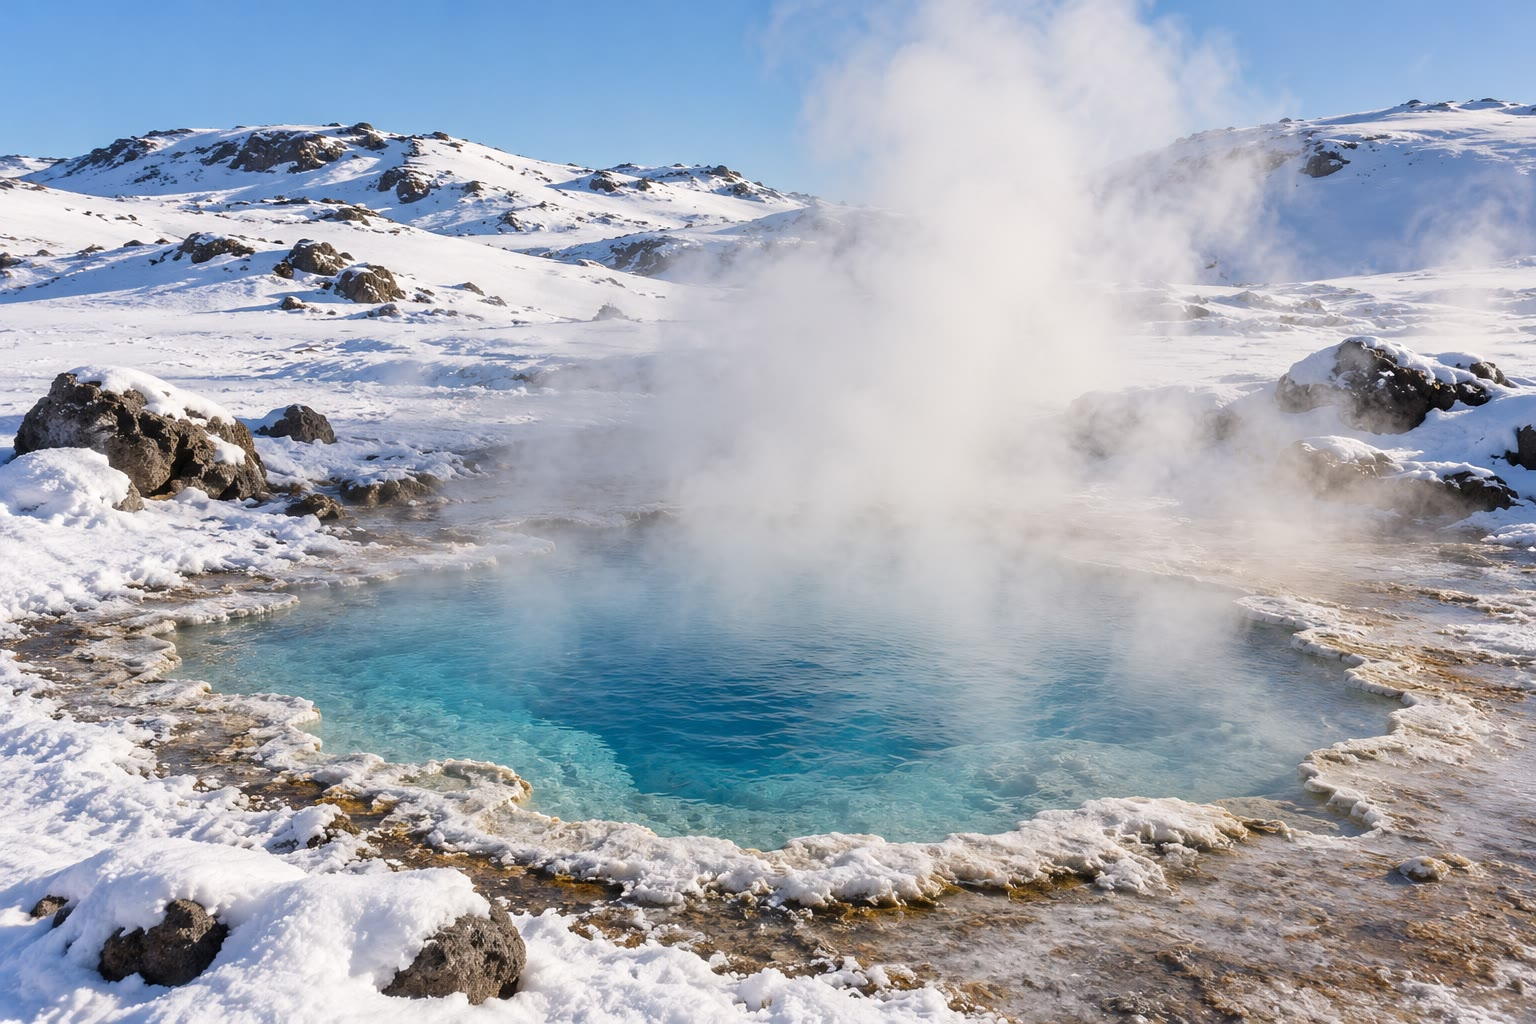
\includegraphics[width=0.6\linewidth]{images/book2/ai/g12-hot-spring-snow.jpg}

{\small Sebuah mata air panas yang beruap di tengah lanskap bersalju: air yang
dipanaskan jauh di bawah tanah kembali ke permukaan (ilustrasi AI).}
\end{omfigure}

\begin{omfigure}
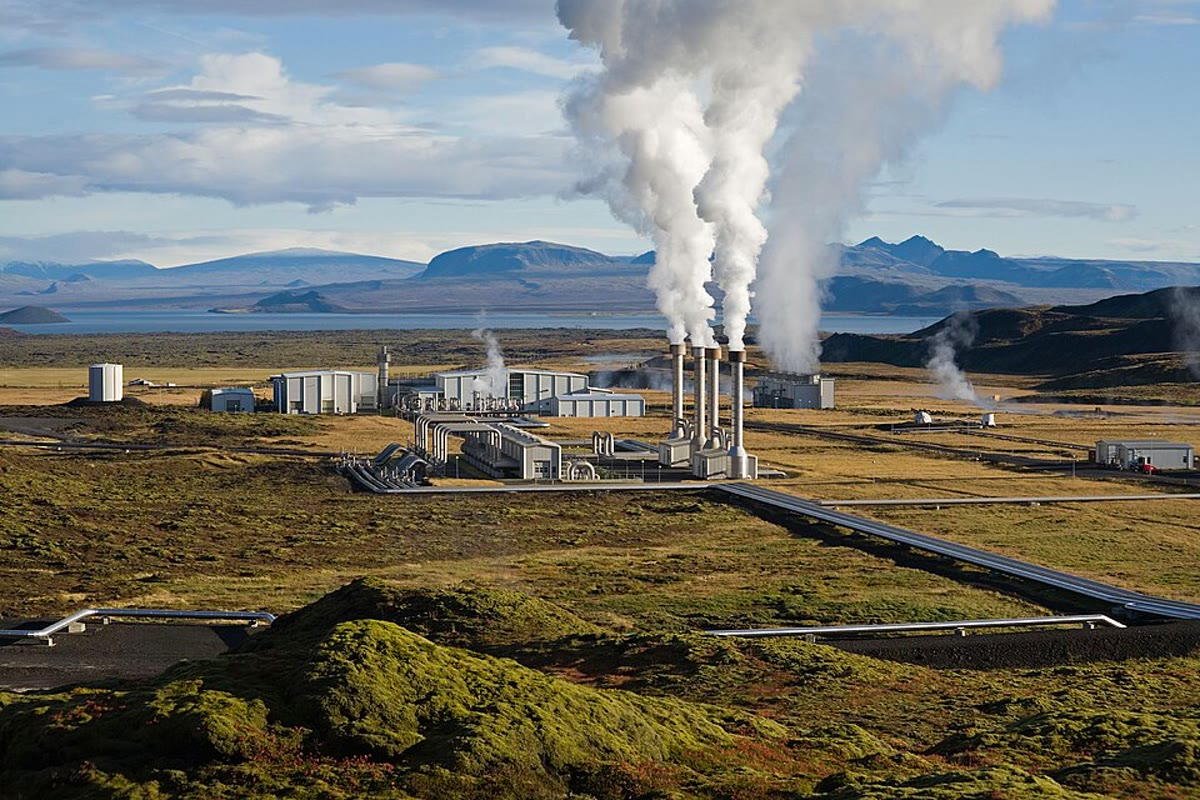
\includegraphics[width=0.66\linewidth]{images/book2/g12-nesjavellir-geothermal.jpg}

{\small Pembangkit listrik panas bumi Nesjavellir, di kawasan vulkanik Hengill
di Islandia: sampai \qty{120}{MW} listrik dan sampai \qty{300}{MW} panas, yang
diangkut oleh air panas. Foto Gretar Ívarsson (domain publik).}
\end{omfigure}
% ledger: photo:g12-nesjavellir, on:nesjavellir

Sebuah lapangan panas bumi tidak tak terbatas pada skala hidup manusia. Di The
Geysers, di California, terlalu banyak sumur menyedot uap, lebih cepat daripada
yang dapat digantikan oleh \omterm{def:g12:internal-heat:heat-flow}{aliran panas} yang lambat dan air hujan: tekanan uap
turun menjadi kurang dari separuh puncaknya, dan lebih dari \qty{40}{\percent}
kapasitas pembangkit-pembangkit listriknya hilang. Kini air disuntikkan kembali
ke dalam lapangan itu untuk memperlambat penurunannya.
% ledger: cpuc:geysers

\section{Latihan}

\begin{exercise}[$\star$]\label{exo:g12:internal-heat:1}
Sebutkan istilahnya: (a) daya yang keluar dari bagian dalam Bumi melalui setiap
meter persegi permukaan; (b) panas yang dilepaskan oleh peluruhan atom-atom
radioaktif dalam satu satuan volume batuan; (c) hilangnya panas yang tersimpan
sejak Bumi terbentuk; (d) perpindahan panas oleh gerak bahan itu sendiri;
(e) panas internal Bumi yang dimanfaatkan manusia.
\end{exercise}

\begin{exercise}[$\star$]\label{exo:g12:internal-heat:2}
Ubahlah: (1) \qty{91.6}{mW/m^2} ke \unit{W/m^2}; (2) \qty{46.7}{TW} ke watt;
(3) \qty{29}{\celsius} per kilometer ke kelvin per meter.
\end{exercise}

\begin{exercise}[$\star$]\label{exo:g12:internal-heat:3}
Sebutkan empat isotop yang menghasilkan hampir seluruh panas radiogenik, dan
katakan dua yang mana yang dapat dilihat oleh detektor KamLAND.
\end{exercise}

\begin{exercise}[$\star$]\label{exo:g12:internal-heat:4}
Dengan $q = 490/\sqrt{t}$, hitung \omterm{def:g12:internal-heat:heat-flow}{aliran panas} melalui dasar samudra yang
berumur 1, 4, 25, dan 49 juta tahun.
\end{exercise}

\begin{exercise}[$\star$]\label{exo:g12:internal-heat:5}
Mengapa \omterm{def:g12:internal-heat:heat-flow}{aliran panas} diukur di dalam lubang bor dan bukan di permukaan itu
sendiri? Mengapa kita harus menunggu setelah pengeboran sebelum mengukur?
\end{exercise}

\begin{exercise}[$\star\star$]\label{exo:g12:internal-heat:6}
Di lubang bor KTB batuan bersuhu sekitar \qty{265}{\celsius} pada
\qty{9.1}{km}. (1) Dengan mengambil \qty{10}{\celsius} di permukaan, hitung
gradien rata-ratanya. (2) Dengan konduktivitas \qty{2.72}{W/(m.K)}, berapa
\omterm{def:g12:internal-heat:heat-flow}{aliran panas} yang dihasilkannya? (3) Bandingkan dengan rata-rata benua.
\end{exercise}

\begin{exercise}[$\star\star$]\label{exo:g12:internal-heat:7}
Benua-benua menutupi \qty{2.073e14}{m^2} dengan \omterm{def:g12:internal-heat:heat-flow}{aliran panas} rata-rata
\qty{70.9}{mW/m^2}, samudra-samudra \qty{3.028e14}{m^2} dengan
\qty{105.4}{mW/m^2}. Hitung daya yang hilang dari masing-masing, jumlahnya,
dan bagian yang hilang melalui dasar samudra.
\end{exercise}

\begin{exercise}[$\star\star$]\label{exo:g12:internal-heat:8}
Lapisan \omterm{def:g12:subduction-magmatism:granodiorite}{granodiorit} setebal \qty{8}{km} mempunyai produksi panas
\qty{1.88}{\micro W/m^3}. (1) Berapa \omterm{def:g12:internal-heat:heat-flow}{aliran panas} yang dihasilkannya di
permukaan? (2) Berapa bagian itu dari \qty{70.9}{mW/m^2}?
\end{exercise}

\begin{exercise}[$\star\star$]\label{exo:g12:internal-heat:9}
Pada umur berapa dasar samudra kehilangan panas sebanyak benua rata-rata,
\qty{70.9}{mW/m^2}, menurut $q = 490/\sqrt{t}$?
\end{exercise}

\begin{exercise}[$\star\star$]\label{exo:g12:internal-heat:10}
Berapa kali lebih banyak panas yang dilepaskan uranium-235 1.4 miliar tahun
yang lalu daripada sekarang? Dan kalium-40, 2.5 miliar tahun yang lalu?
\end{exercise}

\begin{exercise}[$\star\star$]\label{exo:g12:internal-heat:11}
Dengan $t \approx L^2/\kappa$ dan $\kappa = \qty{1e-6}{m^2/s}$, berapa lama
panas melintasi secara konduksi (1) aliran lava setebal \qty{10}{m};
(2) \omterm{def:g11:lithosphere-asthenosphere:lithosphere}{litosfer} setebal \qty{100}{km}; (3) mantel? Nyatakan setiap hasil dalam
satuan yang masuk akal.
\end{exercise}

\begin{exercise}[$\star\star\star$]\label{exo:g12:internal-heat:12}
Saat ini torium-232 melepaskan sekitar \qty{10.4}{TW}, uranium-238
\qty{9.6}{TW}, kalium-40 \qty{4.0}{TW}, dan uranium-235 \qty{0.42}{TW}.
Dengan waktu paruh pada gambar, hitung panas
masing-masing 3 miliar tahun yang lalu, jumlahnya, dan bagian kedua isotop
yang berumur pendek.
\end{exercise}

\begin{exercise}[$\star\star\star$]\label{exo:g12:internal-heat:13}
Pembangkit listrik Nesjavellir dapat menyalurkan sampai \qty{300}{MW} panas,
yang diangkut oleh sekitar \qty{1640}{L} air panas per detik. Dengan kalor
jenis \qty{4180}{J/(kg.K)} dan massa \qty{1}{kg} per liter, berapa derajat air
ini telah dipanaskan? Seberapa luas benua rata-rata yang kehilangan
\qty{300}{MW} panas?
\end{exercise}

\begin{exercise}[$\star\star\star$]\label{exo:g12:internal-heat:14}
Andaikan sebuah lempeng memerlukan 100 juta tahun untuk bergerak dari
punggungan ke palung, dan satu putaran konveksi melalui seluruh mantel sekitar
200 juta tahun. (1)
Bandingkan waktu-waktu ini dengan 260 miliar tahun konduksi melintasi mantel.
(2) Mengapa konveksi dapat mengangkut panas jauh lebih cepat, walaupun mantel
hanya bergerak beberapa sentimeter setahun?
\end{exercise}

\begin{exercise}[$\star\star\star$]\label{exo:g12:internal-heat:15}
Andaikan inti kehilangan sekitar \qty{10}{TW} panas ke dalam mantel melintasi
\omterm{def:g11:seismic-structure:core}{batas inti--mantel}, \qty{2891}{km} di bawah permukaan. (1) Berapa bagian itu
dari \omterm{def:g12:internal-heat:secular-cooling}{pendinginan sekuler}, \qty{22.3}{TW}? Dari mana sisanya
berasal? (2) Hitung \omterm{def:g12:internal-heat:heat-flow}{aliran panas} rata-rata yang melintasi
\omterm{def:g11:seismic-structure:core}{batas inti--mantel}, dan bandingkan dengan \omterm{def:g12:internal-heat:heat-flow}{aliran panas} rata-rata di permukaan,
\qty{91.6}{mW/m^2}. (3) Mengapa inti yang panas dapat menghangatkan dasar
mantel walaupun mantel itu padat?
\end{exercise}

\begin{problem}[{Soal akhir pekan --- Neraca panas Bumi}]
\label{pb:g12:internal-heat:1}
% ledger: b2dd10:continents, b2dd10:half-space, kamland11:geonu, dye12:isotopes, dye12:bse, b2vila:heat-production
% values (internal_heat.py): radiogenic 24.4 TW, secular 22.3 TW, share 0.523, K40 4.0, U235 0.42, U238 9.59
\omterm{def:g12:internal-heat:heat-flow}{Aliran panas} Bumi telah diukur di lebih dari 38\,000 tempat.
Rata-rata benua-benua kehilangan \qty{70.9}{mW/m^2} di atas \qty{2.073e14}{m^2},
dan dasar samudra \qty{105.4}{mW/m^2} di atas \qty{3.028e14}{m^2}.

\medskip
\noindent\textbf{Bagian I --- Aliran panas dan luas.}
\begin{enumerate}
  \item Periksalah bahwa jumlah kedua luas itu sama dengan luas bola yang
        berjari-jari \qty{6371}{km}.
  \item Berapa bagian permukaan yang berupa dasar samudra?
  \item Mengapa dasar samudra kehilangan lebih banyak panas per meter persegi
        daripada benua?
  \item Dengan $q = 490/\sqrt{t}$, hitung \omterm{def:g12:internal-heat:heat-flow}{aliran panas} melalui dasar samudra
        yang berumur 4 juta tahun.
  \item Sebuah lubang bor di granit (\qty{2.72}{W/(m.K)}) mengukur
        \qty{26}{\celsius} per kilometer. Apakah \omterm{def:g12:internal-heat:heat-flow}{aliran panasnya} di atas atau
        di bawah rata-rata benua?
\end{enumerate}

\medskip
\noindent\textbf{Bagian II --- Jumlahnya.}
\begin{enumerate}[resume]
  \item Hitung daya yang hilang melalui benua-benua.
  \item Hitung daya yang hilang melalui dasar samudra.
  \item Jumlahkan keduanya: \omterm{def:g12:internal-heat:heat-flow}{aliran panas} total Bumi, dalam terawatt.
  \item Berapa \omterm{def:g12:internal-heat:heat-flow}{aliran panas} rata-rata di atas seluruh permukaan?
  \item Bila granit setebal \qty{10}{km} (\qty{24.3}{mW/m^2}) terletak di
        bawah setiap benua, berapa terawatt yang akan dihasilkannya? Bandingkan
        dengan daya yang hilang melalui benua-benua.
\end{enumerate}

\medskip
\noindent\textbf{Bagian III --- Panas radiogenik.}
\begin{enumerate}[resume]
  \item KamLAND menghitung geoneutrino dari uranium-238 dan torium-232:
        bersama-sama keduanya melepaskan sekitar \qty{20.0}{TW}, dengan
        \qty{3.9}{kg} torium di Bumi untuk setiap kilogram uranium. Satu
        kilogram uranium melepaskan \qty{94.4}{\micro W} melalui uranium-238-nya
        dan \qty{4.10}{\micro W} melalui uranium-235-nya; satu kilogram torium,
        \qty{26.3}{\micro W}. Hitung panas uranium-238, lalu panas uranium-235.
  \item Kalium-40 menambahkan sekitar \qty{4}{TW}. Hitung panas radiogenik
        totalnya.
  \item Jenis batuan apa yang membawa sebagian besar unsur ini, dan di mana
        batuan itu berada?
  \item Apakah panas radiogenik lebih besar atau lebih kecil 3 miliar tahun
        yang lalu? Mengapa?
\end{enumerate}

\medskip
\noindent\textbf{Bagian IV --- Pendinginan sekuler.}
\begin{enumerate}[resume]
  \item Berapa daya yang tidak dipasok oleh radioaktivitas?
  \item Dari mana daya itu berasal?
  \item Hitung bagian \omterm{def:g12:internal-heat:heat-flow}{aliran panas} yang dipasok oleh \omterm{def:g12:internal-heat:secular-cooling}{pendinginan sekuler}.
  \item Model-model komposisi Bumi memberikan panas radiogenik 11 sampai
        \qty{38}{TW}.
        Di antara bagian berapa saja bagian radiogenik itu kemudian terletak?
  \item Apa yang mengangkut sebagian besar panas ini melalui mantel?
  \item Simpulkan: berapa bagian kehilangan panas Bumi yang dipasok oleh
        radioaktivitas saat ini?
\end{enumerate}
\end{problem}
